\documentclass[11pt,a4paper]{scrreprt}
\usepackage[T1]{fontenc}
\usepackage[utf8]{inputenc}
\usepackage[german,english]{babel}
\usepackage{graphicx}

\begin{document}
\selectlanguage{\german}
\title{\LARGE Design- und Implementationsdokumentation für WeatherInfo}
\author{{\bf SE3 Team}\\Tobias Koenig}
\date{Juni 2009}

\maketitle

\tableofcontents

\chapter{Einleitung}
Im Anschluss an die Analysephase, deren Ergebnisse im Dokument analyse.pdf
zusammengefasst sind, wurden in der Designphase der grobe und feine
Aufbau des Beispielprogramms WeatherInfo entwickelt. Da das Model-View-Controller
Konzept ein integraler Bestandteil der Applikation darstellt, wurde der
grobe Aufbau dadurch implizit schon festgelegt. Der Feinentwurf definierte
die einzelnen Komponenten des Programms, welche eine nahezu 1:1 Repr\"asentation
im Quellcode haben, und die Kommunikation zwischen ihnen.

\chapter{Der Grobwurf}
Das Programm l\"asst sich grob in drei Module unterteilen:
\begin{itemize}
  \item \textbf{Views} Das Views-Modul enth\"alt alle visuellen Komponenten des Programms
                       und definiert welche Interaktion zwischen den Komponenten stattfinden kann.
  \item \textbf{Model} Das Model-Modul enth\"alt das Daten-Model und die Datenstrukturen, welche
                       zur Kommunikation zwischen dem Model-Modul und Storage-Modul ben\"otigt werden.
  \item \textbf{Storage} Das Storage-Modul enth\"alt die Komponenten welche zum Laden der Daten vom
                         WebService ben\"otigt werden.
\end{itemize}

\begin{center}
  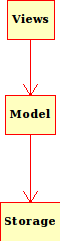
\includegraphics[width=2cm]{grobentwurf.png}
\end{center}

\chapter{Der Feinentwurf}
Im Feinentwurf wurde der Grobentwurf dahingehend \"uberarbeitet, dass das Views-Modul
jetzt in die einzelnen View-Komponenten zerlegt wurde und die Beziehungen zwischen ihnen
verdeutlicht. So stellt die {\itshape MainWidget} Komponente das Hauptfenster dar, aus
dem heraus die anderen Views aktiviert werden k\"onnen. Sowohl das {\itshape MainWidget}
als auch die anderen Views haben eine Assoziation zu dem {\itshape WeatherModel}, welches
den Model Aspekt des MVC in diesem Programm wiederspiegelt. Das {\itshape WeatherModel}
seinerseits hat eine Assoziation zum {\itshape AbstractStorage} bzw. einem seiner beiden
konkreten Implementierungen {\itshape StaticStorage} oder {\itshape WebStorage}.
Diese beiden Komponenten sind daf\"ur verantwortlich die Wetterdaten aus einem lokalen
Speicher bzw. aus dem Internet zu Laden und an das {\itshape WeatherModel} zu \"ubergeben.
Als Containerstruktur f\"ur diese Daten wird {\itshape WeatherSet} verwendet.

\begin{center}
  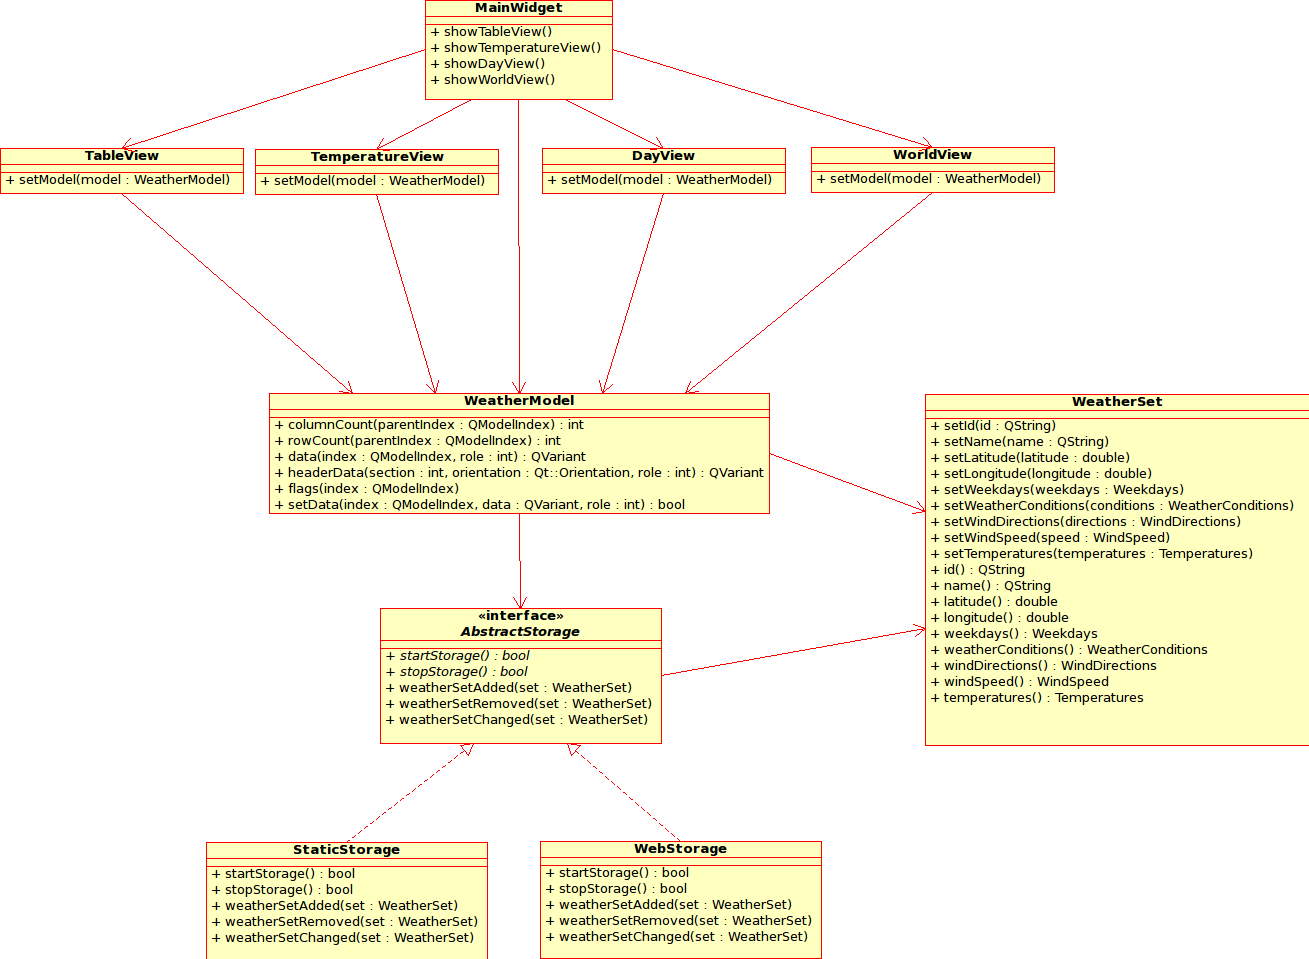
\includegraphics[width=14cm]{feinentwurf.png}
\end{center}

Im Diagramm ist zu sehen, dass eine Assoziation vom Storage zum Model, bzw. vom Model
zu den Views fehlt. Das ist dem Umstand geschuldet, dass der Datenaustausch bzw. die
Benachrichtigung \"uber Daten\"anderungen nicht \"uber Funktionsaufrufe realisiert wird,
und damit der Empf\"anger der Daten und dessen Schnittstelle bekannt sein muss, sondern
\"uber den Signal/Slot-Mechanismus des Qt-Frameworks, welcher eine Bindung der Komponenten
zur Laufzeit gestattet. Dadurch wird eine zus\"atzliche Entkopplung zwischen den Komponenten
erreicht und im Gegensatz zum original MVC Paradigma muss das Model keine Informationen
\"uber den View besitzen, der View entscheidet gegen welches Model er sich bindet und auf
welche Signale er reagieren m\"ochte.

\chapter{Die Implementation}
Die Entwicklung des Programms wurde basierend auf dem Qt-Framework durchgef\"uhrt,
welches es erm\"oglicht, plattform\"ubergreifende Software in C++ zu implementieren.
Neben Funktionen zum Anzeigen von Fenstern und Malen von Graphiken beinhaltet es ein
Model-View-Framework, was den modularen Entwurf und Implementierung von Programmen
zum Anzeigen von Daten aus verschiedenen Datenquellen in unterschiedlichen Ansichten
erheblich vereinfacht. Das {\itshape MainWidget} und die verschiedenen Views wurden
von {\itshape QWidget} abgeleitet und haben damit eine visuelle Repr\"asentation auf
dem Bildschirm. {\itshape WeatherModel} ist eine Subklasse von {\itshape QAbstractTableModel},
welches wiederum von {\itshape QAbstractItemModel} ist und damit das Basis-Interface
des Qt Model-View-Frameworks zur Verf\"ugung stellt. Eine konkrete Implementation von
{\itshape QAbstractItemModel} kann man an verschiedenste Klassen des Qt-Frameworks
\"ubergeben, welche die Daten unterschiedlich darstellen. {\itshape QTableView} listet
die Daten in einer Tabelle auf, wohingegen {\itshape QListView} nur die erste Spalte
des Models in einer Liste darstellt. {\itshape QComboBox} wiederum bietet dem Benutzer an,
die Daten einer definierten Spalte des Models aus einer Drop-Down Box auszuw\"ahlen.
In WeatherInfo wurde von den vordefinierten Views nur {\itshape QTableView} f\"ur die
Tabellenansicht der Wetterdaten verwendet.

Eine weitere verwendete Funktionalit\"at des Qt-Frameworks sind die Proxy-Models.
Diese Klassen, welche von {\itshape QAbstractProxyModel} erben, bekommen ein {\itshape QAbstractItemModel}
als Source-Model und bieten selbst ebenfalls das Interface des {\itshape QAbstractItemModel}
an. Sie k\"onnen damit zwischen einer datenbasierten {\itshape QAbstractItemModel} Implementation und
einem View geschoben werden und Filter-, Sortier- oder Struktur\"anderungsfunktionen \"ubernehmen.
WeatherInfo macht davon Gebrauch um die Anzeige der St\"adte in der Tabellenansicht zu
filtern.
\end{document}
